% !TeX spellcheck = en_US
%\documentclass[11pt,a4paper]{article}
\documentclass[11pt
  , a4paper
  , article
  , oneside
%  , twoside
%  , draft
]{memoir}

\usepackage{control}
\usepackage{kotex}
\usepackage[numbers]{natbib}
%\usepackage[pdftex]{graphicx}
%\DeclareGraphicsExtensions{.pdf,.png,.jpg}
\begin{document}

\newcommand{\technumber}{
  Digital Signal Processing using MATLAB\\
  Document 1: 2016-03-26}
\title{\textbf{Digital Signal Processing: 실습 2 \\
		제2장 이산시간 신호 및 시스템 \\}}

\author{이상일\thanks{silee7103@ibs.re.kr} \\

  학번: 201460437\\
  Computer Engineering, Chungnam National University 
}
\date{\today}

\renewcommand{\maketitlehooka}{\begin{flushright}\textsf{\technumber}\end{flushright}}
%\renewcommand{\maketitlehookb}{\centering\textsf{\subtitle}}
%\renewcommand{\maketitlehookc}{C}
%\renewcommand{\maketitlehookd}{D}

\maketitle

\begin{abstract}
MATLAB을 사용한 Digital Signal Processing에 대한 실습과제에 대한 Documents를 구성한다.
\end{abstract}

\chapter{Example 2-1:}

\section{2-1-1}

\begin{lstlisting}[style=termstyle]
n=[-5:5];
x = 2 * impseq(-2,-5,5) - impseq(4,-5,5);
subplot(2,2,1);
stem(n,x); title('Sequence in Problem 2.1a');
xlabel('n'); ylabel('x(n)');
\end{lstlisting}

\section{2-1-2}

\begin{lstlisting}[style=termstyle]
n=[0:20];
x1 = n.*(stepseq(0,0,20) - stepseq(10,0,20));
x2 = 10*exp(-0.3*(n-10)).*(stepseq(10,0,20)-stepseq(20,0,20));
x = x1+x2;
subplot(2,2,2);
stem(n,x); title('Sequence in Problem 2.1b');
xlabel('n'); ylabel('x(n)');
\end{lstlisting}

\section{2-1-3}
\begin{lstlisting}[style=termstyle]
n=[0:50];
x = cos(0.04*pi*n) + 0.2*randn(size(n));
subplot(2,2,3);
stem(n,x); title('Sequence in Problem 2.1c');
xlabel('n'); ylabel('x(n)');
\end{lstlisting}

\section{2-1-4}
\begin{lstlisting}[style=termstyle]
n=[-10:9];
x = [5,4,3,2,1];
xtilde = x' * ones(1, 4); xtilde = (xtilde(:))';
subplot(2,2,4);
stem(n,xtilde); title('Sequence in Problem 2.1d');
xlabel('n'); ylabel('xtilde(n)');
\end{lstlisting}

\begin{figure}[h!]
	\centering
	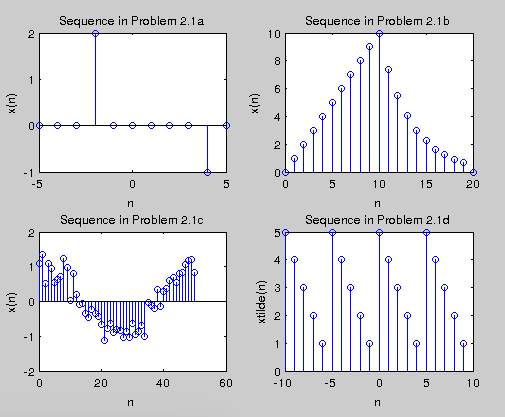
\includegraphics{./images/ex2-1.png}
	\caption{Example 2.1 Result}
	\label{fig:Example 2.1 Result} 
\end{figure}

\chapter{Example 2-2:}

\section{2-2-1}

\begin{lstlisting}[style=termstyle]
[x11,n11]=sigshift(x,n,5); [x12,n12]=sigshift(x, n, -4);
[x1, n1]= sigadd(2*x11, n11, -3*x12, n12);
subplot(2,1,1);
stem(n1,x1); title('Sequence in Example 2.2a');
xlabel('n'); ylabel('x1(n)');
\end{lstlisting}

\section{2-2-2}
\begin{lstlisting}[style=termstyle]
[x21,n21]=sigfold(x,n); [x21,n21]=sigshift(x21, n21, 3);
[x22,n22]= sigshift(x,n,2); [x22,n22]=sigmult(x,n,x22,n22);
[x2,n2]= sigadd(x21,n21, x22,n22);
subplot(2,1,2);
stem(n2,x2); title('Sequence in Example 2.2b');
xlabel('n'); ylabel('x2(n)');
\end{lstlisting}

\begin{figure}[h!]
	\centering
	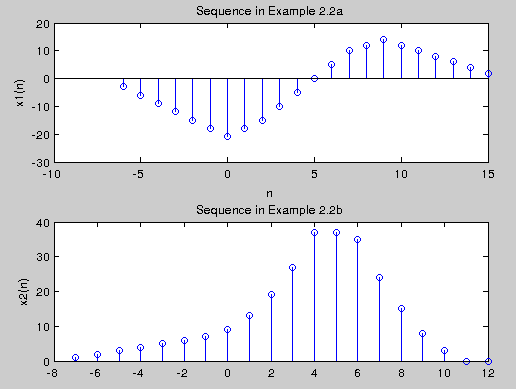
\includegraphics{./images/ex2-2.png}
	\caption{Example 2.2 Result}
	\label{fig:Example 2.2 Result} 
\end{figure}

\chapter{Example 2-3: }

\begin{lstlisting}[style=termstyle]
n=[-10:1:10]; alpha = -0.1+0.3j;
x = exp(alpha*n);
subplot(2,2,1); stem(n, real(x)); title('Real part'); xlabel('n');
subplot(2,2,2); stem(n, imag(x)); title('Imaginary part'); xlabel('n');
subplot(2,2,3); stem(n, abs(x)); title('Magnitude part'); xlabel('n');
subplot(2,2,4); stem(n, (180/pi)*angle(x)); title('Phase part'); xlabel('n');
\end{lstlisting}

\begin{figure}[h!]
	\centering
	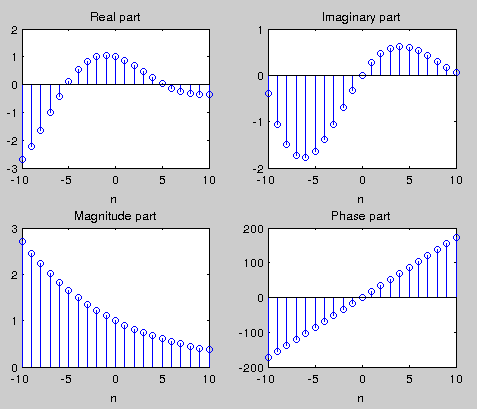
\includegraphics{./images/ex2-3.png}
	\caption{Example 2.3 Result}
	\label{fig:Example 2.3 Result} 
\end{figure}

\chapter{Example 2-4:}
\begin{lstlisting}[style=termstyle]
n=[0:10]; x = stepseq(0,0,10)-stepseq(10,0,10);
[xe,xo,m]=evenodd(x,n);

subplot(2,2,1); stem(n,x); title('Rectangura pulse');
xlabel('n'); ylabel('x(n)'); axis([-10,10,0,1.2]);

subplot(2,2,2); stem(m,xe); title('Even Part');
xlabel('n'); ylabel('xe(n)'); axis([-10,10,0,1.2]);

subplot(2,2,4); stem(m,xo); title('Odd Part');
xlabel('n'); ylabel('xo(n)'); axis([-10,10,-0.6,0.6]);
\end{lstlisting}

\begin{figure}[h!]
	\centering
	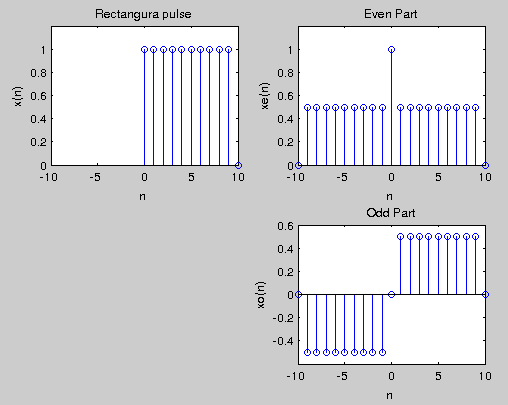
\includegraphics{./images/ex2-4.png}
	\caption{Example 2.4 Result}
	\label{fig:Example 2.4 Result} 
\end{figure}

%\hfill\break

\chapter{Example 2-7:}

\begin {equation}
h(n) = (0.9)^n u(n) 
\end {equation}
에 대한 출력 y(n) 을 구하라.\\
풀이)

\begin {equation}
y(n) = \displaystyle\sum_{k=0}^{9} (1)(0.9)^{(n-k)}u(n-k)=(0.9)^n\displaystyle\sum_{k=0}^{9}(0.9)^{-k}u(n-k)
\end {equation}

\section{경우 1.}
n $<$ 0 인 경우, \\
\begin {equation}
y(n) = 0
\end {equation}
x(n)과 h(n)의 0이 아닌 값들은 겹치지 않는다.

\section{경우 2.}
0 $<= $ n $<$ 9 인 경우, \\
\begin {equation}
y(n) = (0.9)^n\displaystyle\sum_{k=0}^{n}(0.9)^{-k}=10[1-(0.9)^{n+1}],  0 \leq n < 9
\end {equation}
임펄스 응답 h(n)은 입력 x(n) 에 일부 겹치는 구간이 발생한다.

\section{경우 3.}
n $>= $ 9 인 경우, \\
\begin {equation}
y(n) = (0.9)^n\displaystyle\sum_{k=0}^{n}(0.9)^{-k}=10(0.9)^{n-9}[1-(0.9)^{10}],  n \geq 9
\end {equation}
임펄스 응답 h(n)은 입력 x(n) 에 완전히 겹친다.

\chapter{Example 2-8:}
\begin{lstlisting}[style=termstyle]
x = [3, 11, 7, 0, -1, 4, 2]; nx =[-3:3];
h = [2, 3, 0, -5, 2, 1]; nh = [-1:4];
[y,ny] = conv_m(x,nx,h,nh);
y
ny
\end{lstlisting}
\begin{figure}[h!]
	\centering
	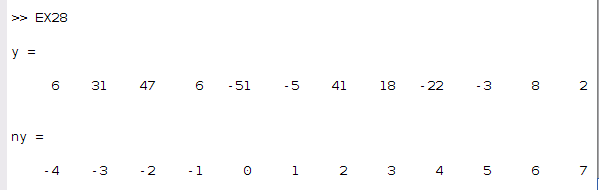
\includegraphics{./images/ex2-8.png}
	\caption{Example 2.8 Result}
	\label{fig:Example 2.8 Result} 
\end{figure}

\end{document}

